\section{Esperimenti e risultati}

\subsection{Scelta delle quantità}


\subsection{Presentazione dei risultati}
In questa sezione si riportano tutti quanti i grafici dei risultati sperimentali. Si cerca di analizzarli per determinarne l'andamento. I grafici \textit{a}, \textit{b} e \textit{c} di ogni sezione riportano le misurazioni effettuate per i singoli test, mentre il grafico \textit{d} riporta tutte le misurazioni assieme al fine di facilitare il confronto.


\subsubsection*{Ingresso Lineare}

Il risultato più significativo di questa batteria di test è rappresentato dalla figura \ref{fig:d_linear_input_combined}, nella quale si osserva chiaramente come, nel caso di inserimento di valori strettamente crescenti, la struttura basata su \textit{Albero Binario di Ricerca} presenti un comportamento analogo a quello della lista ordinata. Nel caso della lista ordinata, ogni nuovo elemento deve essere inserito in coda e ciò richiede l'attraversamento di tutti gli elementi già presenti; di conseguenza, il costo di una singola operazione di inserimento cresce linearmente rispetto al numero di elementi memorizzati.

In modo analogo, un \textit{Albero Binario di Ricerca} alimentato con valori strettamente crescenti degenera progressivamente in una struttura lineare, in cui ogni nodo possiede solamente il figlio destro. L'altezza dell'albero diventa quindi pari a $n$ e ogni operazione di inserimento richiede l'attraversamento di tutti i nodi precedentemente inseriti, producendo anch'essa un andamento lineare rispetto alla dimensione della struttura.

Diverso è invece il comportamento dell'\textit{AVL}. Grazie alle operazioni di bilanciamento e rotazione, l'altezza dell'albero rimane sempre logaritmica rispetto al numero di elementi memorizzati. Di conseguenza, anche nel caso peggiore di input ordinato, il costo delle operazioni di inserimento rimane pari a $O(\log n)$. Sebbene dai grafici tale andamento possa apparire quasi lineare, ciò è dovuto principalmente alla lenta crescita della funzione logaritmica e alle dimensioni relativamente contenute dell'input utilizzato nei test.

\begin{figure}[H]
	\centering
	\begin{subfigure}[b]{0.47\textwidth}
		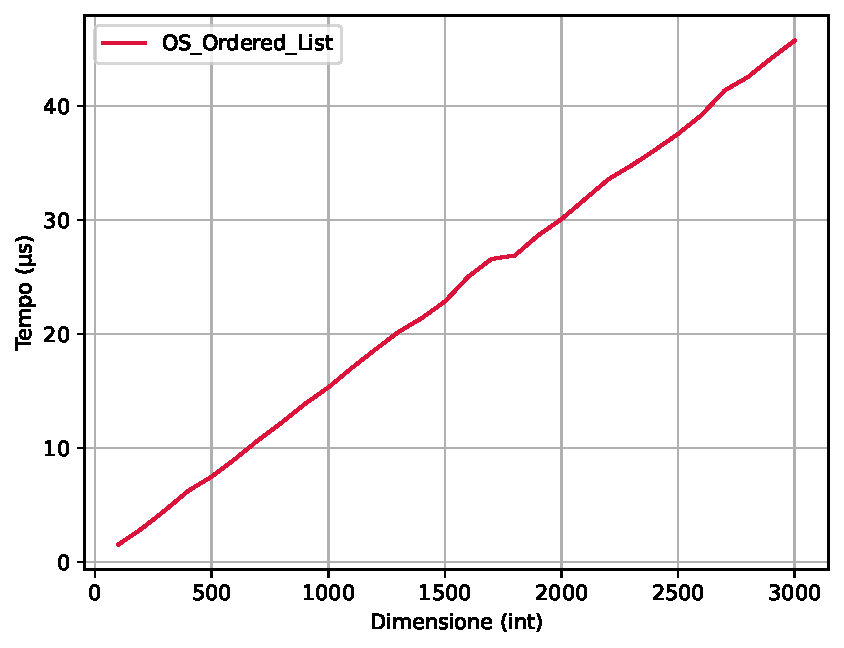
\includegraphics[width=\textwidth]{figures/results/figures/test_linear_input_OS_Ordered_List.pdf}
		\caption{Lista Ordinata}
		\label{fig:a_linear_input_OS_Ordered_List}
	\end{subfigure}
	\begin{subfigure}[b]{0.47\textwidth}
		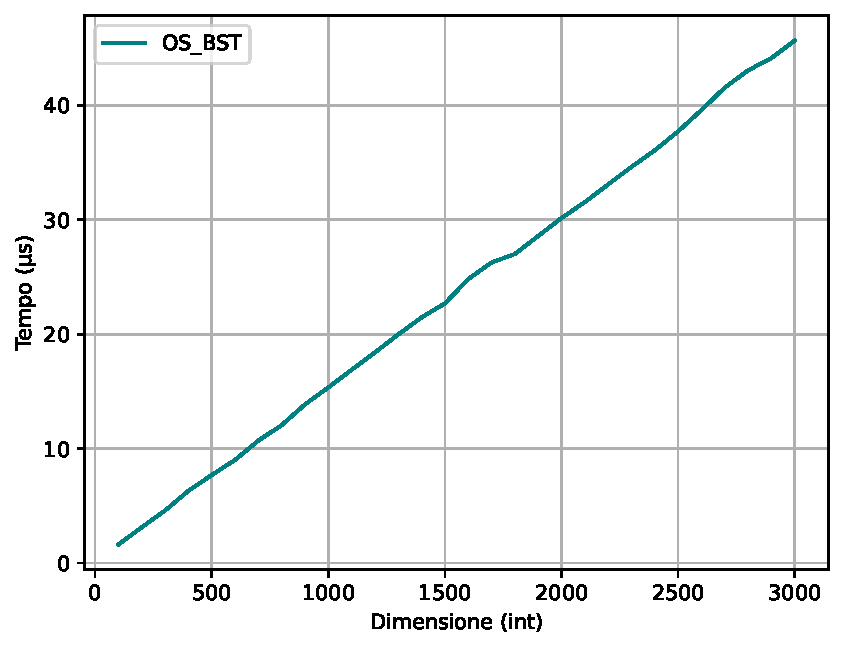
\includegraphics[width=\textwidth]{figures/results/figures/test_linear_input_OS_BST.pdf}
		\caption{ABR}
		\label{fig:b_linear_input_OS_BST}
	\end{subfigure}
	\begin{subfigure}[b]{0.47\textwidth}
		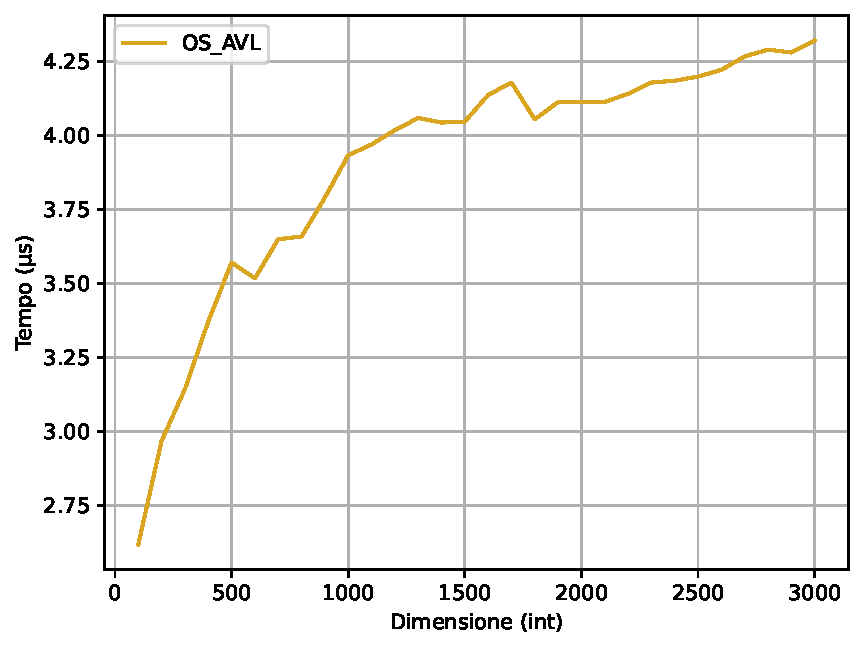
\includegraphics[width=\textwidth]{figures/results/figures/test_linear_input_OS_AVL.pdf}
		\caption{AVL}
		\label{fig:c_linear_input_OS_AVL}
	\end{subfigure}
	\begin{subfigure}[b]{0.47\textwidth}
		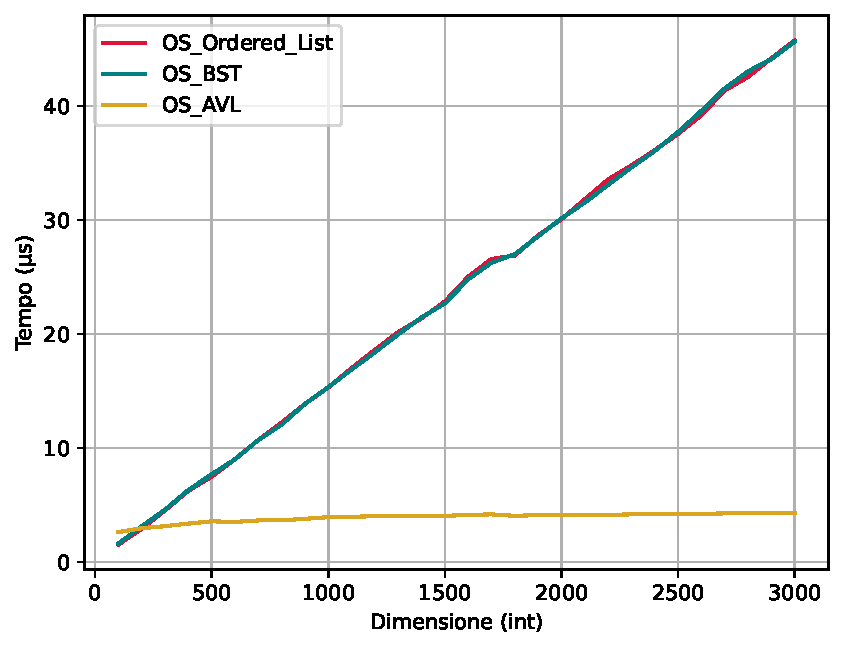
\includegraphics[width=\textwidth]{figures/results/figures/test_linear_input_combined.pdf}
		\caption{Totale}
		\label{fig:d_linear_input_combined}
	\end{subfigure}
	\caption{Andamento con ingresso lineare}
	\label{fig:input_lineare}
\end{figure}

\subsubsection*{Ingresso Casuale}

Nel test di inserimento casuale, riportato in figura \ref{fig:d_casual_input_combined}, sia l'\textit{AVL} sia l'\textit{ABR} mostrano un andamento molto simile e nettamente migliore rispetto alla lista ordinata. Questo comportamento è giustificato dal fatto che, con input casuali, l'\textit{ABR} tende mediamente a mantenere una struttura sufficientemente bilanciata, ottenendo quindi un'altezza prossima a $\log n$. Di conseguenza, il costo medio delle operazioni di inserimento risulta anch'esso prossimo a $O(\log n)$.

Si osserva inoltre come l'\textit{ABR} risulti in alcuni intervalli leggermente più efficiente dell'\textit{AVL}. Tale differenza è dovuta principalmente all'overhead introdotto dalle operazioni di bilanciamento dell'\textit{AVL}, come l'aggiornamento delle altezze, delle dimensioni dei sottoalberi e le eventuali rotazioni. La lista ordinata, invece, continua a presentare un andamento lineare crescente, poiché ogni inserimento richiede mediamente l'attraversamento di una parte significativa della struttura.

\begin{figure}[H]
	\centering
	\begin{subfigure}[b]{0.47\textwidth}
		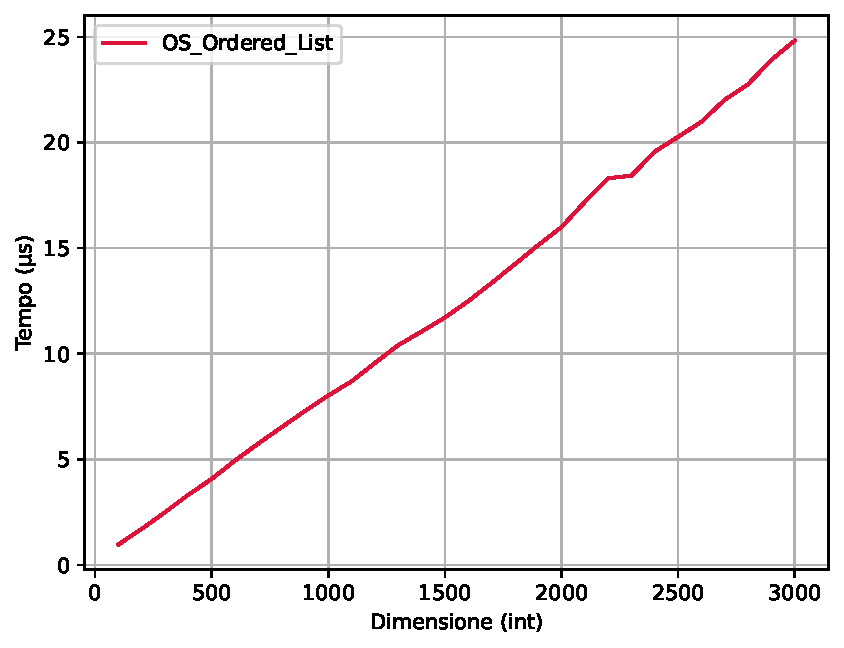
\includegraphics[width=\textwidth]{figures/results/figures/test_casual_input_OS_Ordered_List.pdf}
		\caption{Lista Ordinata}
		\label{fig:a_casual_input_OS_Ordered_List}
	\end{subfigure}
	\begin{subfigure}[b]{0.47\textwidth}
		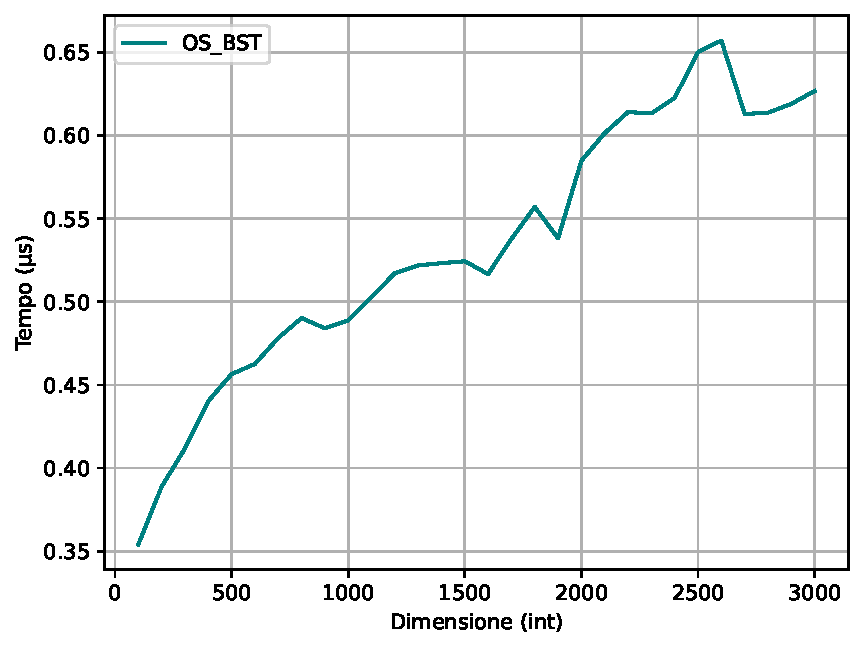
\includegraphics[width=\textwidth]{figures/results/figures/test_casual_input_OS_BST.pdf}
		\caption{ABR}
		\label{fig:b_casual_input_OS_BST}
	\end{subfigure}
	\begin{subfigure}[b]{0.47\textwidth}
		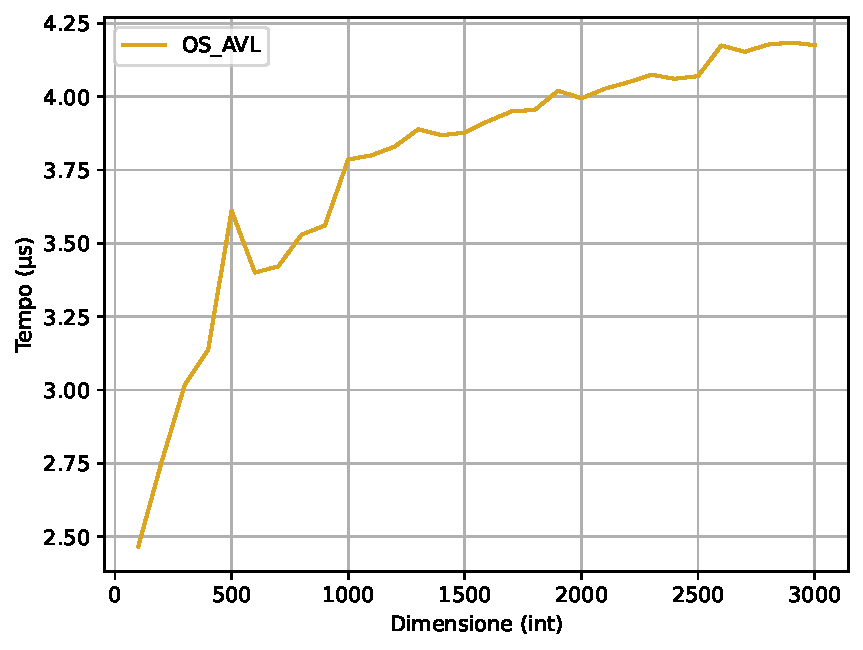
\includegraphics[width=\textwidth]{figures/results/figures/test_casual_input_OS_AVL.pdf}
		\caption{AVL}
		\label{fig:c_casual_input_OS_AVL}
	\end{subfigure}
	\begin{subfigure}[b]{0.47\textwidth}
		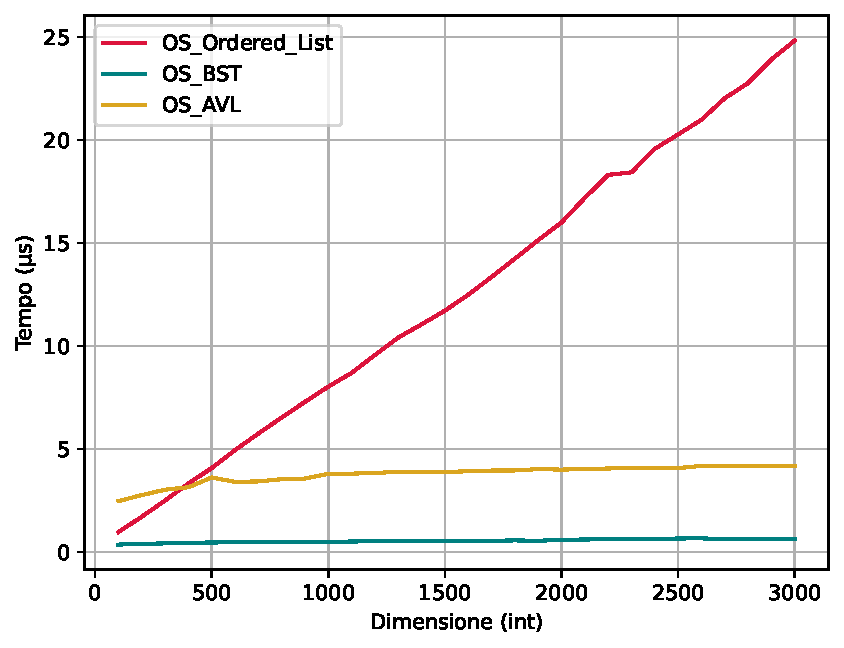
\includegraphics[width=\textwidth]{figures/results/figures/test_casual_input_combined.pdf}
		\caption{Totale}
		\label{fig:d_casual_input_combined}
	\end{subfigure}
	\caption{Andamento con ingresso casuale}
	\label{fig:_lineare}
\end{figure}

\subsubsection*{Cancellazione Casuale}

Nel test di cancellazione casuale, riportato in figura \ref{fig:d_casual_deletion_combined}, sia l'\textit{AVL} sia l'\textit{ABR} mostrano un andamento simile e nettamente migliore rispetto alla lista ordinata. Questo comportamento è dovuto al fatto che le strutture vengono inizialmente popolate con valori casuali e risultano quindi mediamente bilanciate. In tali condizioni, le operazioni di ricerca del nodo da eliminare richiedono un tempo medio prossimo a $O(\log n)$.

La lista ordinata, invece, necessita di una scansione lineare per individuare ciascun elemento da rimuovere. Di conseguenza, anche il costo medio delle operazioni di eliminazione cresce linearmente rispetto alla dimensione della struttura, producendo una curva significativamente più accentuata rispetto a quelle ottenute con le strutture ad albero.

\begin{figure}[H]
	\centering
	\begin{subfigure}[b]{0.47\textwidth}
		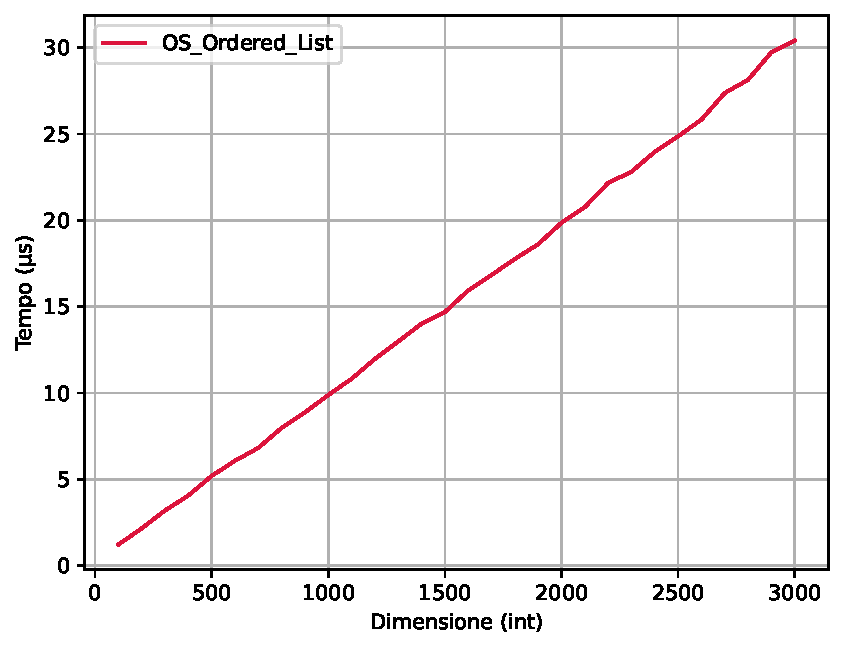
\includegraphics[width=\textwidth]{figures/results/figures/test_casual_deletion_OS_Ordered_List.pdf}
		\caption{Lista Ordinata}
		\label{fig:a_casual_deletion_OS_Ordered_List}
	\end{subfigure}
	\begin{subfigure}[b]{0.47\textwidth}
		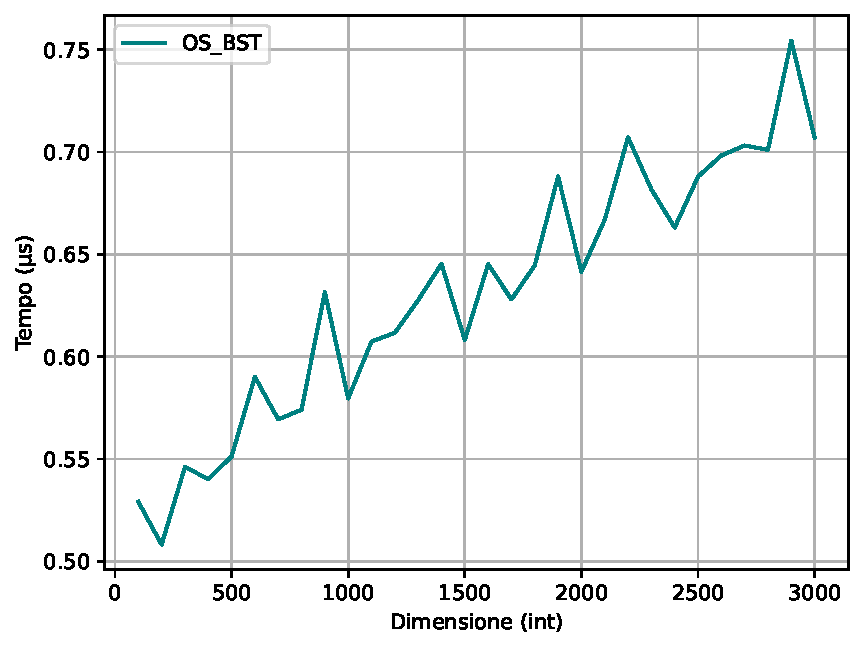
\includegraphics[width=\textwidth]{figures/results/figures/test_casual_deletion_OS_BST.pdf}
		\caption{ABR}
		\label{fig:b_casual_deletion_OS_BST}
	\end{subfigure}
	\begin{subfigure}[b]{0.47\textwidth}
		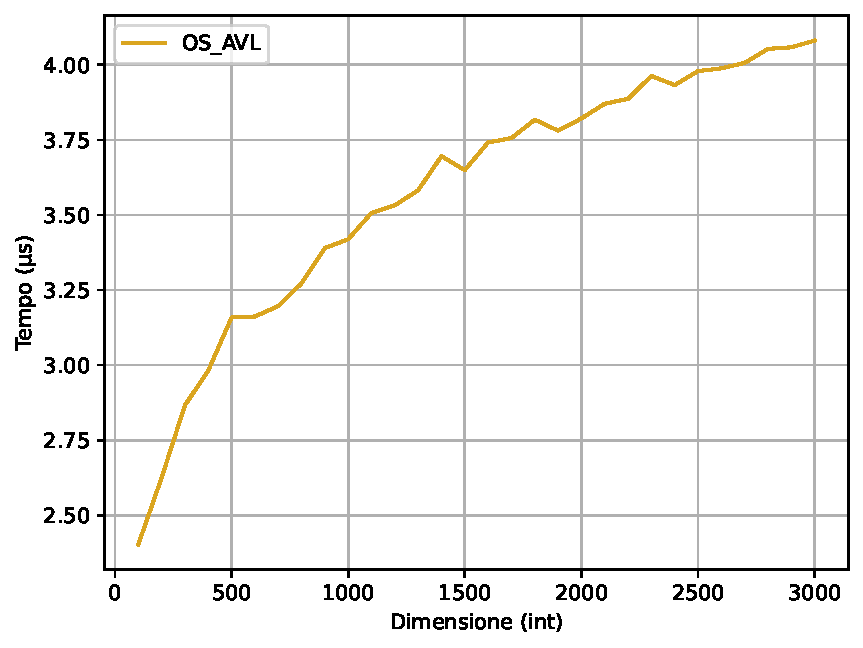
\includegraphics[width=\textwidth]{figures/results/figures/test_casual_deletion_OS_AVL.pdf}
		\caption{AVL}
		\label{fig:c_casual_deletion_OS_AVL}
	\end{subfigure}
	\begin{subfigure}[b]{0.47\textwidth}
		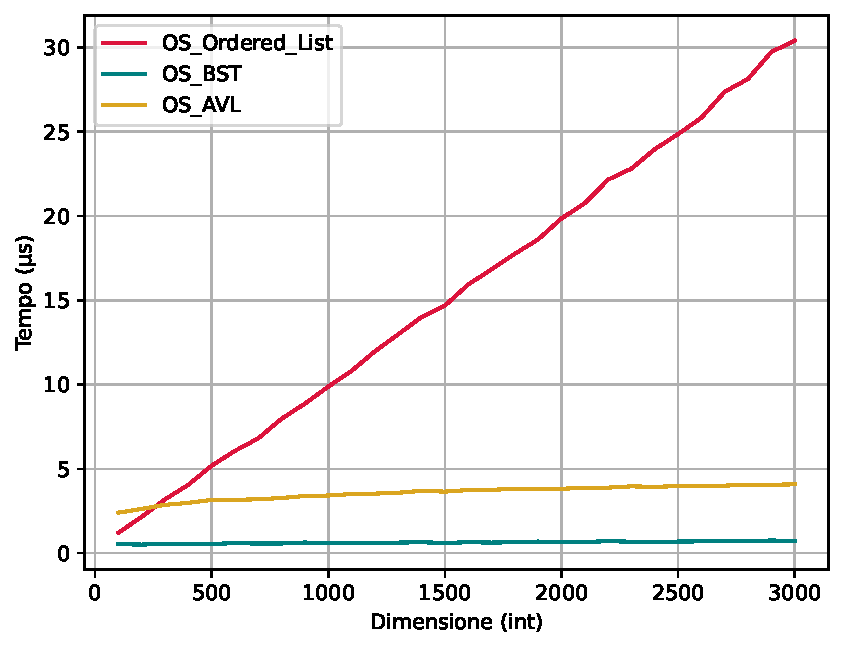
\includegraphics[width=\textwidth]{figures/results/figures/test_casual_deletion_combined.pdf}
		\caption{Totale}
		\label{fig:d_casual_deletion_combined}
	\end{subfigure}
	\caption{Andamento eliminazione casuale}
	\label{fig:deletion_lineare}
\end{figure}

\subsubsection*{Ranking e Selezione Casuali}

I test relativi alle operazioni di \textit{rank} e \textit{select}, illustrati nelle figure \ref{fig:d_casual_rank_combined} e \ref{fig:d_casual_selection_combined}, evidenziano in maniera particolarmente marcata la superiorità dell'\textit{AVL}. In questa implementazione, infatti, ogni nodo mantiene l'informazione relativa alla dimensione del proprio sottoalbero; ciò consente di calcolare sia il rango di un elemento sia l'$i$-esimo elemento ordinato in tempo $O(\log n)$.

Nel caso dell'\textit{ABR}, invece, le operazioni \textit{rank} e \textit{select} richiedono il ricalcolo ricorsivo della dimensione dei sottoalberi tramite la funzione \texttt{\_size()}, aumentando significativamente il costo delle operazioni. Sebbene l'albero risulti mediamente bilanciato grazie all'inserimento casuale dei valori, il continuo ricalcolo delle dimensioni introduce un overhead aggiuntivo che rende le prestazioni sensibilmente peggiori rispetto a quelle ottenute con l'\textit{AVL}.



\begin{figure}[H]
	\centering
	\begin{subfigure}[b]{0.47\textwidth}
		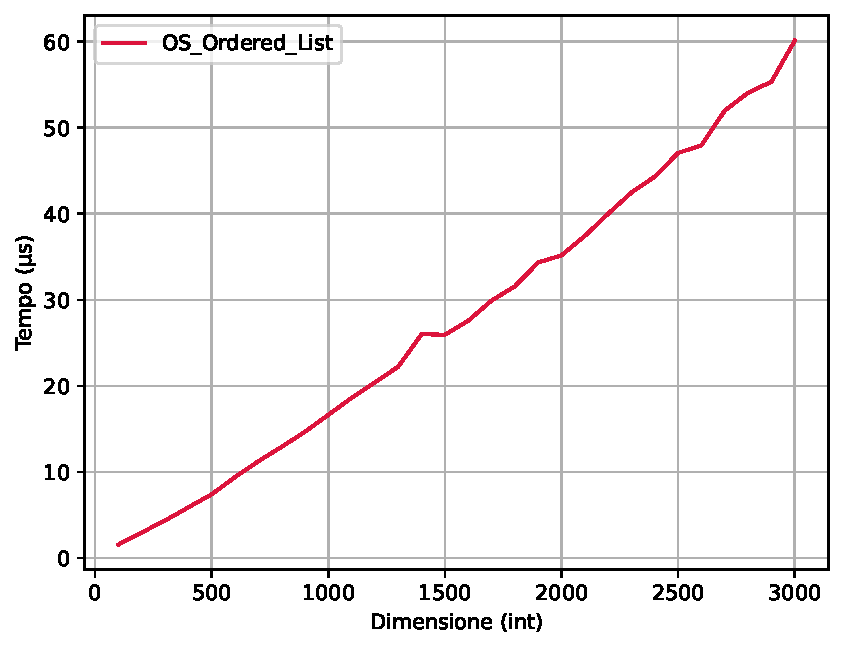
\includegraphics[width=\textwidth]{figures/results/figures/test_casual_rank_OS_Ordered_List.pdf}
		\caption{Lista Ordinata}
		\label{fig:a_casual_rank_OS_Ordered_List}
	\end{subfigure}
	\begin{subfigure}[b]{0.47\textwidth}
		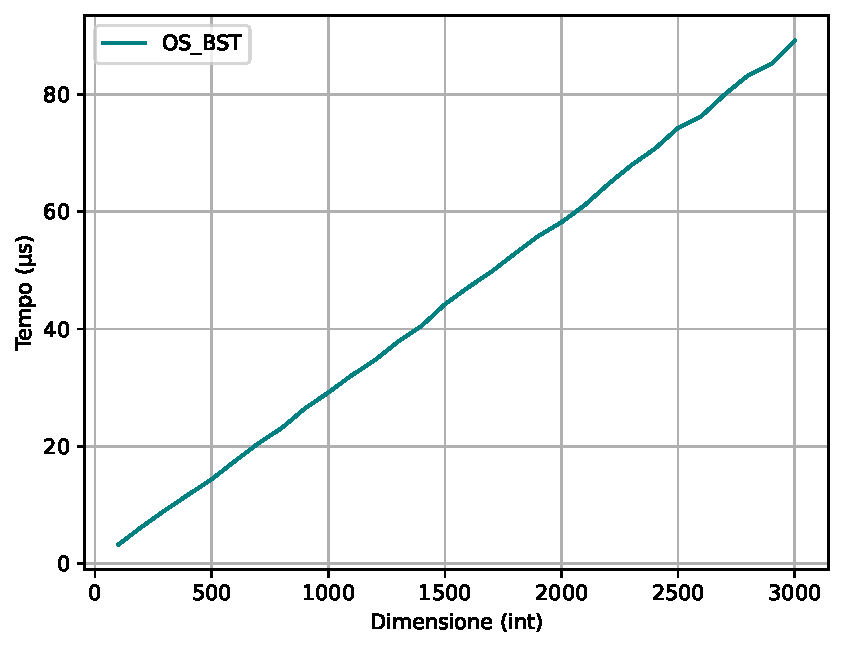
\includegraphics[width=\textwidth]{figures/results/figures/test_casual_rank_OS_BST.pdf}
		\caption{ABR}
		\label{fig:b_casual_rank_OS_BST}
	\end{subfigure}
	\begin{subfigure}[b]{0.47\textwidth}
		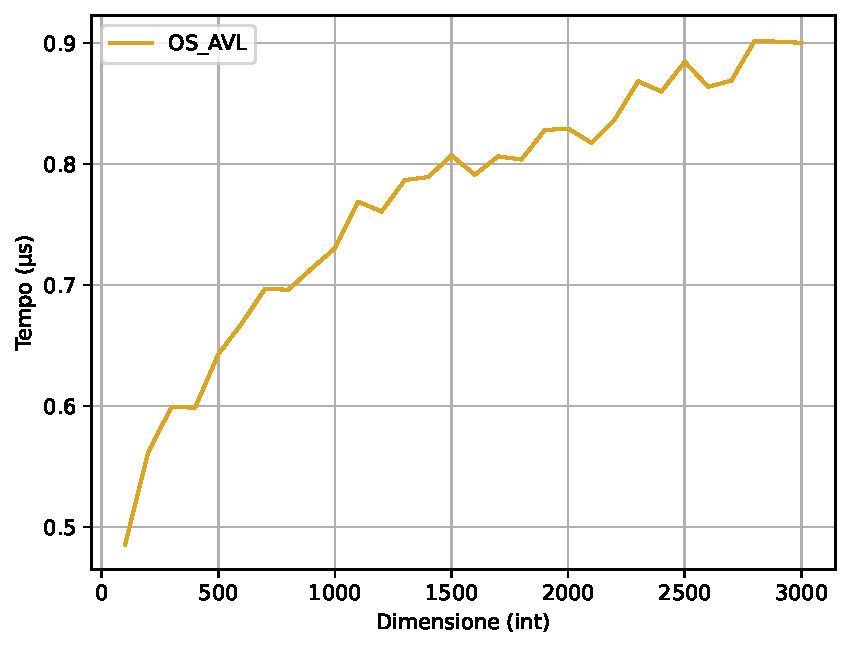
\includegraphics[width=\textwidth]{figures/results/figures/test_casual_rank_OS_AVL.pdf}
		\caption{AVL}
		\label{fig:c_casual_rank_OS_AVL}
	\end{subfigure}
	\begin{subfigure}[b]{0.47\textwidth}
		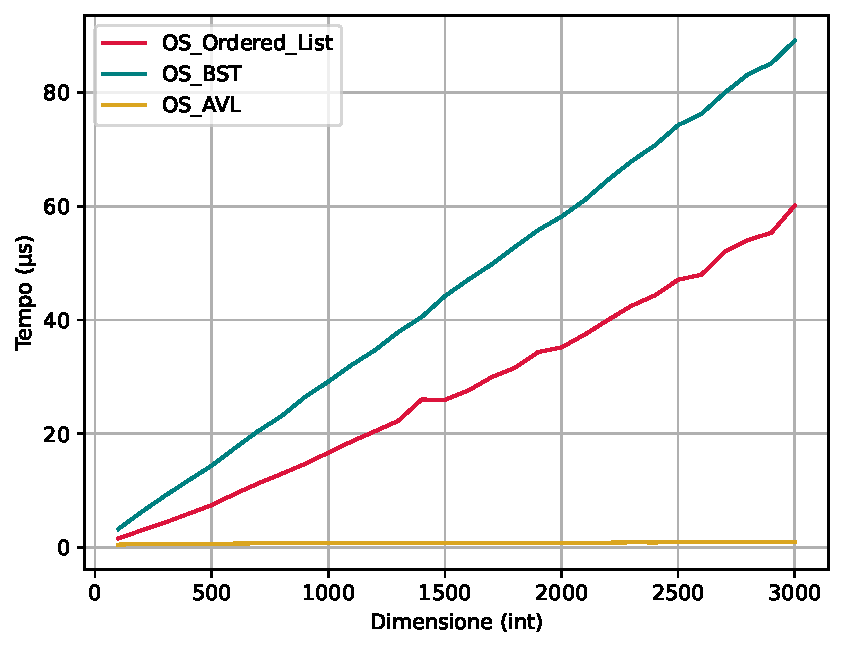
\includegraphics[width=\textwidth]{figures/results/figures/test_casual_rank_combined.pdf}
		\caption{Totale}
		\label{fig:d_casual_rank_combined}
	\end{subfigure}
	\caption{Andamento ranking casuale}
	\label{fig:rank_lineare}
\end{figure}

In particolare, nel test di \textit{select} si osservano forti oscillazioni nel grafico relativo all'\textit{ABR}. Questo fenomeno è dovuto principalmente alla natura casuale delle query effettuate e alla diversa struttura dei sottoalberi attraversati durante l'esecuzione dell'algoritmo. Infatti, la funzione \texttt{select()} può richiedere il calcolo della dimensione di sottoalberi molto differenti tra loro a seconda del valore richiesto; di conseguenza, il costo delle singole operazioni può variare sensibilmente tra un'esecuzione e l'altra. Tali oscillazioni risultano quindi compatibili sia con l'assenza di un meccanismo di bilanciamento rigoroso sia con il ricalcolo ricorsivo delle dimensioni dei sottoalberi.

\begin{figure}[H]
	\centering
	\begin{subfigure}[b]{0.47\textwidth}
		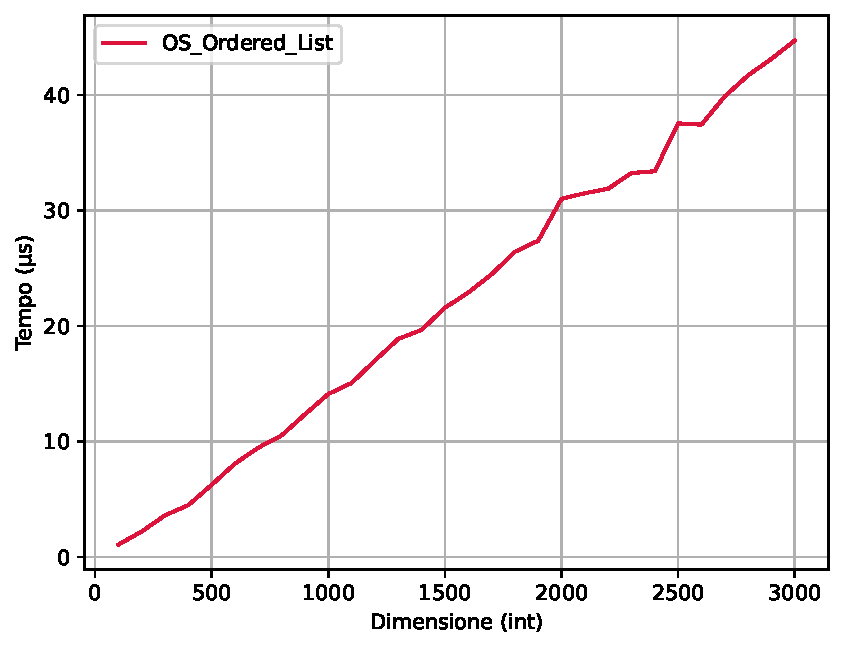
\includegraphics[width=\textwidth]{figures/results/figures/test_casual_selection_OS_Ordered_List.pdf}
		\caption{Lista Ordinata}
		\label{fig:a_casual_selec_OS_Ordered_List}
	\end{subfigure}
	\begin{subfigure}[b]{0.47\textwidth}
		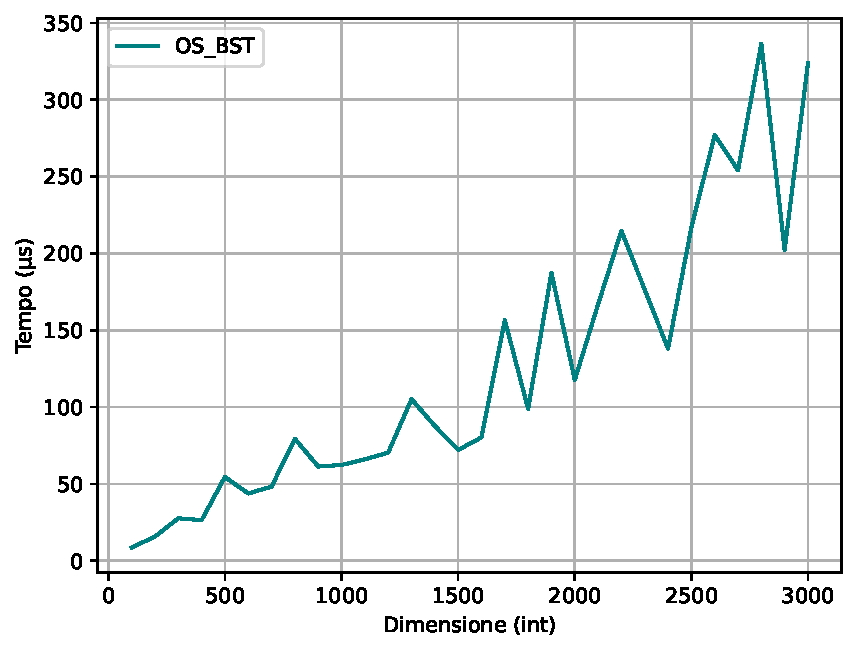
\includegraphics[width=\textwidth]{figures/results/figures/test_casual_selection_OS_BST.pdf}
		\caption{ABR}
		\label{fig:b_casual_selection_OS_BST}
	\end{subfigure}
	\begin{subfigure}[b]{0.47\textwidth}
		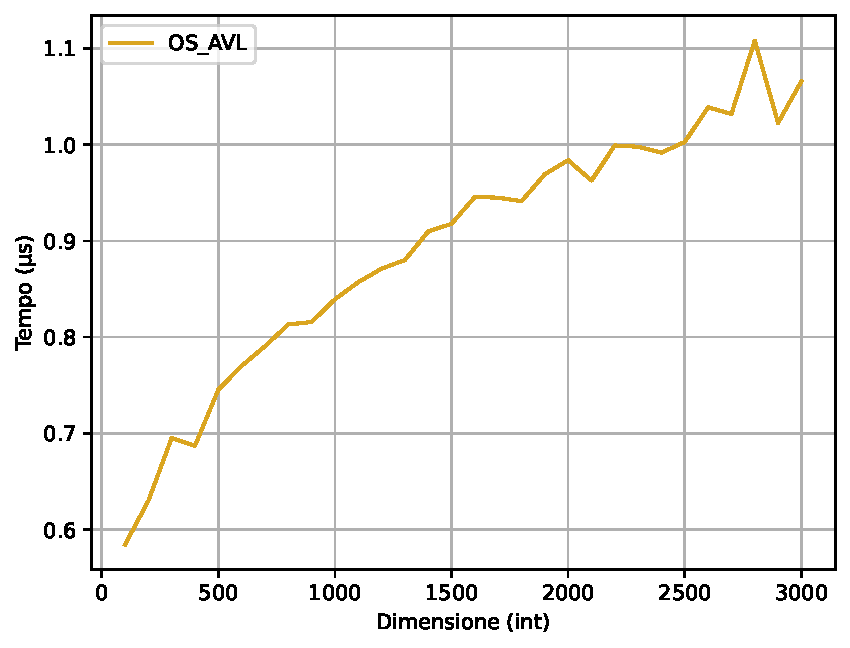
\includegraphics[width=\textwidth]{figures/results/figures/test_casual_selection_OS_AVL.pdf}
		\caption{AVL}
		\label{fig:c_casual_selection_OS_AVL}
	\end{subfigure}
	\begin{subfigure}[b]{0.47\textwidth}
		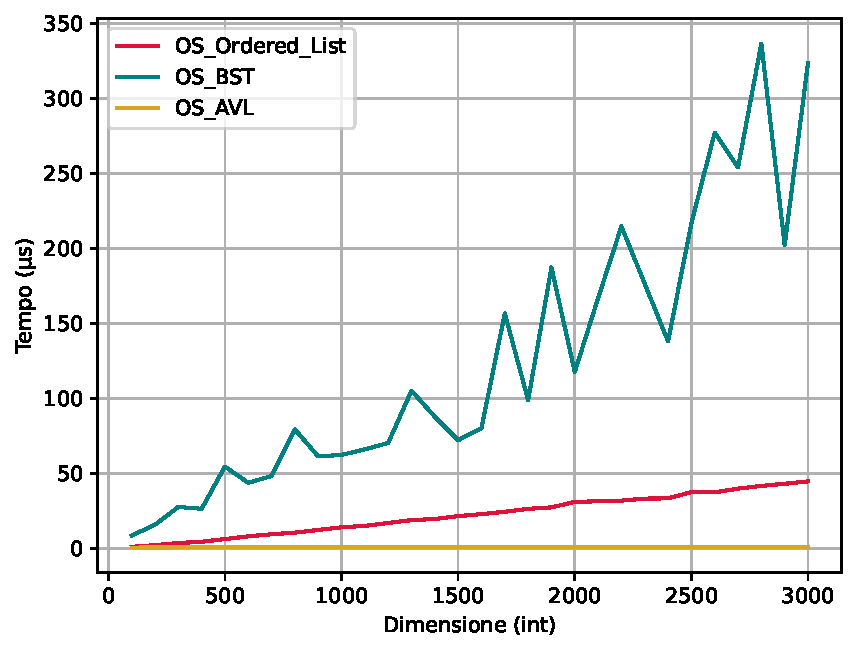
\includegraphics[width=\textwidth]{figures/results/figures/test_casual_selection_combined.pdf}
		\caption{Totale}
		\label{fig:d_casual_selection_combined}
	\end{subfigure}
	\caption{Andamento selezione casuale}
	\label{fig:seleszione_lineare}
\end{figure}

\newpage